% Chapter 3

\chapter{Implementation} % Write in your own chapter title
\label{Chapter3}
\lhead{Chapter 3. \emph{Implementation}} % Write in your own chapter title to set the page header

\orange
\begin{shaded}
SPolly in its entirety is a compound of three parts. The first one is called 
region speculation and it is embedded into Polly. The second and the third 
part are Sambamba modules, one for the compile time and the other one
for the runtime. The region speculation part acts like a storage and interface
for all discovered sSCoPs, thus it contains most of the transformation code.
The Sambama passes concentrate on the program 
\begin{wraptable}[]{r}{0.45\textwidth}
  \caption{Lines of code for Polly, SPolly and Sambamba components}
  \begin{center}
    \begin{tabular}{ l r }
     component     & LOC  \\
      \hline
      SPolly     & XXX \\
      ~ Region Speculation     & XXX \\
      ~ SPolly Sambama CT  & XXX \\
      ~ SPolly Sambama RT  & XXX \\
      Polly     & XXX \\
      ~ SCoP Detection     & XXX \\
      ~ Code Generation    & XXX \\
      Sambamba     & XXX \\
      ~ Parallelizer     & XXX \\
               TODO MORE & \\
    \end{tabular}
  \end{center}
  \label{tab:LinesOfCode}
\end{wraptable}
logic which is at the moment 
far more evolved in the runtime part. The compile time component plays a minor
role but it can be enriched by new functionalities in the future. Beyond the 
three parts of SPolly I implemented a basic Profiler and Statistics module for
Sambamba which have been very helpful during the development and may become 
permanent features of Sambama as there are any comparable counterparts at the 
moment. During the implementation various bugs occurred and even if most of them
arose through my own fault I triggered some in the code base of Polly and 
Sambamba too. A full table of reported bugs is listed in table 
\ref{tab:Bugreports}. Table \ref{tab:LinesOfCode} compares the work in a
quantitative manner as it lists the lines of code (LOC) added for SPolly as well
as for Sambama and Polly parts.
[TODO one sentence about the table content]

[TODO rephrase] 
Table \ref{tab:CommandLineOptions} lists all available command line options 
added in the context of SPolly. Although all of these options work 
without the Sambamba modules, yet Sambama at all, the last three would only 
produce sequential executable code without any parallelization. 
[TODO] As for now I am not quite sure if this could be of any practical use, 
but to my understanding Polly could get a similar option in the near future. 





\section{Speculative Polly}
It would be feasible to look at SPolly as extension to Polly, especially designed
to interact with Sambamba. As such it was crucial to preserve all functionality 
of Polly and supplement it with (mostly speculative) new ones. Most of them are
implemented in the region speculation, but there are some new options in the 
code generation too. Apart from these two locations the SCoP detection was the 
only component which has been touched. It is ideally suited to serve as the 
bridge between Polly and the speculative part as speculative valid regions 
would be rejected here. The information currently needed for region speculation
is also available at this point and can be directly reused.

As the Polly architecture is nicely illustrated by figure 
\ref{fig:PollyArchitecture}, it has been extended in figure 
\ref{fig:SPollyArchitecture} to capture the changes introduced by SPolly. 
In comparison the region speculation, the fork join backend and the sSCoP
backend have been added as they can be used without Sambamba. 
\end{shaded}

\begin{figure}[htbp]
  \centering
  \includegraphics[width=0.9\textwidth]{Primitives/SPollyArchitecture.png}
  \caption{SPolly architecture}
  \label{fig:SPollyArchitecture}  
\end{figure}

\begin{shaded}

\subsection{Region Speculation}
The region speculation (RS) of SPolly has several tasks to fulfill. The first 
one includes the communication with Polly or more precise, 
with the SCoP detection. Each region analyzed by the SCoP detection needs to be
considered as possibly speculative valid SCoPs, thus all information exposed 
during the detection are stored. If the region contains a validation not 
listed in \ref{tab:ValidationsSpeculatedOn} or if it is without any validation
the information are discarded, else a new sSCoP is created which initially 
validates itself. These validation mainly computes information needed for later
transformations. In the following these computations as well as the creation of 
profiling and parallel versions for a sSCoP are explained briefly.


\subsubsection{Region Scores}

\lstset{frame=none}
\begin{wrapfigure}[]{r}{0.4\textwidth}
  \centering
  \subfloat[complete static sSCoP]{
    \lstinputlisting{Primitives/Code/sSCoPstatic.c}
    \label{lst:sSCoPstatic}  
  }

  \subfloat[Branch within a sSCoP]{
    \lstinputlisting{Primitives/Code/sSCoPbranch.c}
    \label{lst:sSCoPbranch}  
  }

  \subfloat[irreversible call within a sSCoP]{
    \lstinputlisting{Primitives/Code/sSCoPprintf.c}
    \label{lst:sSCoPprintf}  
  }
  \caption{example sSCoPs}
  \label{fig:ScoredSCoPs}
\end{wrapfigure}
\resetlst

Region scores are the heuristic used to decide which sSCoPs may be interesting
to speculate on, thus for which region should profiling and parallel versions
be created and used. As the former ones may change the score again it is 
reasonable to create parallel version later if the collected data suggest to do
so. Initial efforts to create these scores did not use any kind of 
memory, thus every call needed to reconsider the whole region. To avoid this
unnecessary computations the current score is a symbolic value which may contain
variables for variables not known statically, branch probabilities and the 
introduced tests. Evaluation of these symbolic values will take all profiling
information into account and yield a comparable integer value. 
Only during the initial region score creation region speculation will
[TODO word! traverse?]. All instructions will be scored and the violating ones
will be checked for their speculative potential.
As memory instructions are 
guarded by the STM for the case the speculation failed, calls may not be
reversible, thus without any speculative potential at all. Such function calls
are not checked earlier since the region speculation needs the information about
possible other branches within this region. Listing \ref{lst:sSCoPprintf} 
provides such an example but these cases will be revisited in the next 
two chapters too. Table \ref{tab:Scores} lists the scores for the examples in 
figure \ref{fig:ScoredSCoPs}. 

\end{shaded}

\begin{table}[htbp]
  \centering
  \caption{Scores for the sSCoPs presented in various listings}
  \begin{tabular}{ c l}
    listing & score \\
    \hline
    \ref{lst:sSCoPstatic} & $ 576 \hfill \text{  (if \texttt{A,B} and \texttt{C} may alias)} $ \\
    \ref{lst:sSCoPbranch} & $63 * (11 + ((7 * \text{@if.then\_ex\_prob}) / 100) + ((5 * \text{@if.else\_ex\_prob}) / 100)) $ \\
    \ref{lst:sSCoPprintf} & $((0\text{ smax }\%\text{N}) / 16) * (6 + (-1000 * \text{@if.then\_ex\_prob} / 100)$ \\
   \end{tabular}
  \label{tab:Scores}
\end{table}

\red
\begin{shaded}
\subsubsection{Memory Accesses}

\subsubsection{Aliasing}

\subsubsection{Non Invariantcy}

\subsubsection{SCoP extraction}

\subsubsection{Profiling Versions}

\subsubsection{Parallel Versions}

\end{shaded}

\orange
\begin{shaded}
\subsection{Code Generation}
As part of the extension of Polly a new code generation type was added. Apart 
from sequential, vectorized and OpenMP annotated code generation SPolly is 
capable of creating a unrolled and blocked loop, which can be easily 
translated into an ParCFG, thus parallelized by a Sambama module. Listing 
\ref{lst:ForkJoinCodeGenerationOUT} presents this transformation. The special 
case where lower and upper bound as well as the 
stride are statically known constants, the second loop, which computes 
remaining iterations, is completely unrolled.
This kind of loop unrolling and blocking may find its 
way into Polly in the near future. 

\subsubsection*{Parallelization}

In order to secure the speculative executions with Sambambas STM
(see \ref{SambambaSTM}) the Sambama parallelizer needs to be used.
As this parallelizer does not yet support loop parallelization per se, some 
transformation needed to be done first. The new code generation type was created
to do the difficult one without recomputing information provided during by the
polytope model (during the code generation) anyway. As these transformation
yields code as in listing \ref{lst:ForkJoinCodeGenerationOUT} the creation of
a ParCFG (see \ref{SambambaParCFG}) remains. Figures \ref{fig:ForkJoinCFG} and
\ref{fig:ForkJoinParCFG} visualize these changes.

\end{shaded}

\lstset{frame=none}
\begin{figure}[htbp]
  \centering
  \subfloat[source]{
    \lstinputlisting{Primitives/Code/ForkJoinCodeGenerationSRC.c}
    \label{lst:ForkJoinCodeGenerationSRC}
  }
  \qquad
  \subfloat[after N-fork creation]{
    \lstinputlisting{Primitives/Code/ForkJoinCodeGenerationOUT.c}
    \label{lst:ForkJoinCodeGenerationOUT}
  }

  \subfloat[SPolly forked CFG]{
    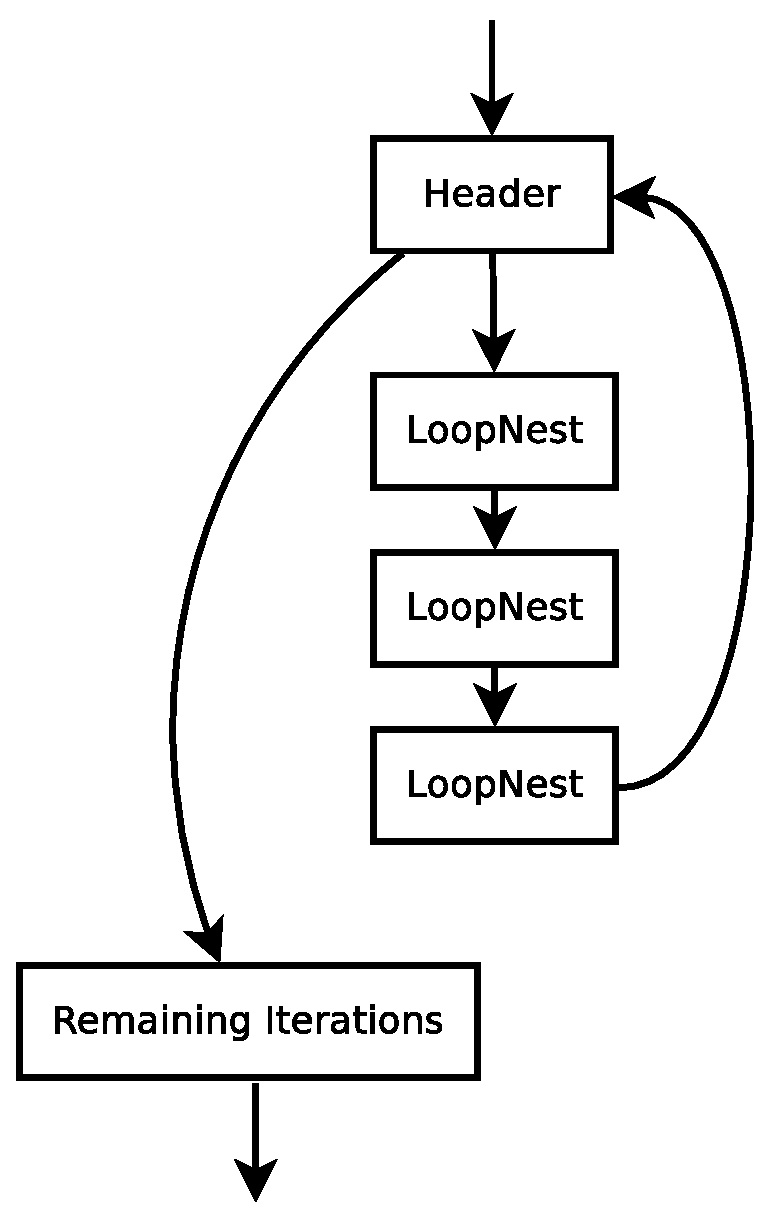
\includegraphics[width=0.27\textwidth]{Figures/ForkJoinCFG.eps}
    \label{fig:ForkJoinCFG} 
  }
  \qquad
  \subfloat[SPolly ParCFG]{
    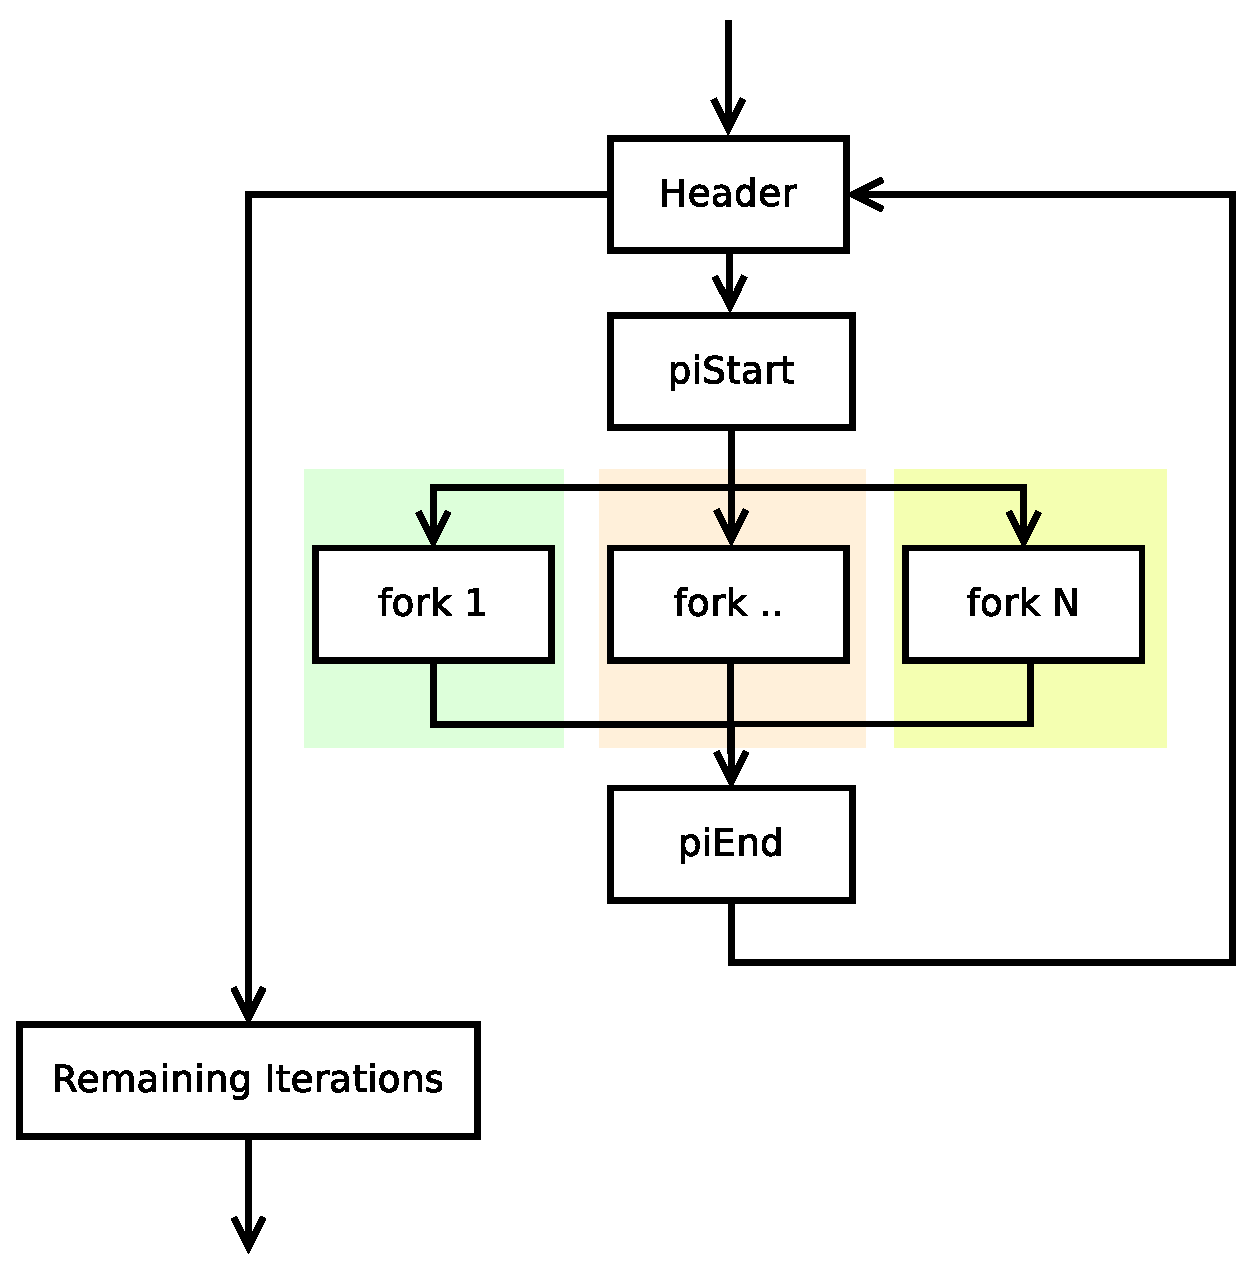
\includegraphics[width=0.63\textwidth]{Figures/ForkJoinParCFG.eps}
    \label{fig:ForkJoinParCFG}
  }
  \caption{Forked CFG produced by SPolly and resulting ParCFG}
  \label{fig:CreateParCFG}  
\end{figure}
\resetlst

\begin{shaded}
\subsection{Introduced tests}
To reduce the overhead of misspeculation tests are introduced in front of
each sSCoP. At the moment there are two different kinds available, 
invariants tests and alias tests. Only the later one is used in optimized 
versions because the former one needs to check the invariant
every iteration, thus it produces a huge overhead. In contrast to profiling 
versions which uses both tests to refine the score of a sSCoP.
Placing the test section was quite easy, since
Polly itself introduces a (constant) branch before the SCoP anyway. Figure
\ref{fig:PollySCoPCFG} and \ref{fig:SPollySCoPCFG} shows the (simplified) 
CFG introduced by Polly and SPolly, respectively. The dotted edge in the CFG
produced by Polly is not taken (constant false), but remains in the CFG. As far
as I know, SPolly is the first extension to Polly which uses the untouched 
original SCoP.

\end{shaded}

\begin{figure}[htbp]
  \centering
  \subfloat[Polly CFG]{
  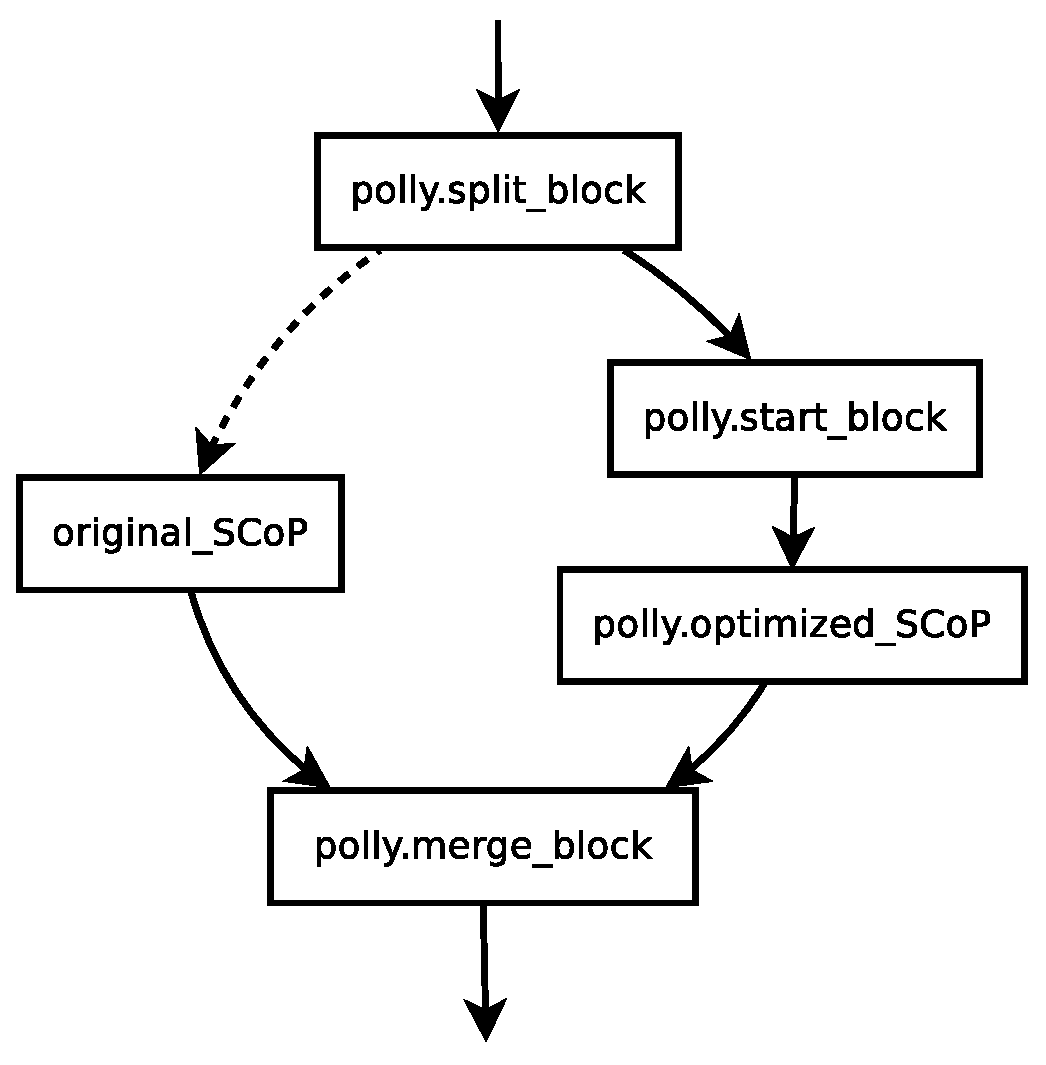
\includegraphics[width=0.45\textwidth]{Figures/PollySCoPCFG.eps}
  \label{fig:PollySCoPCFG}}
  \subfloat[SPolly optimized CFG]{
  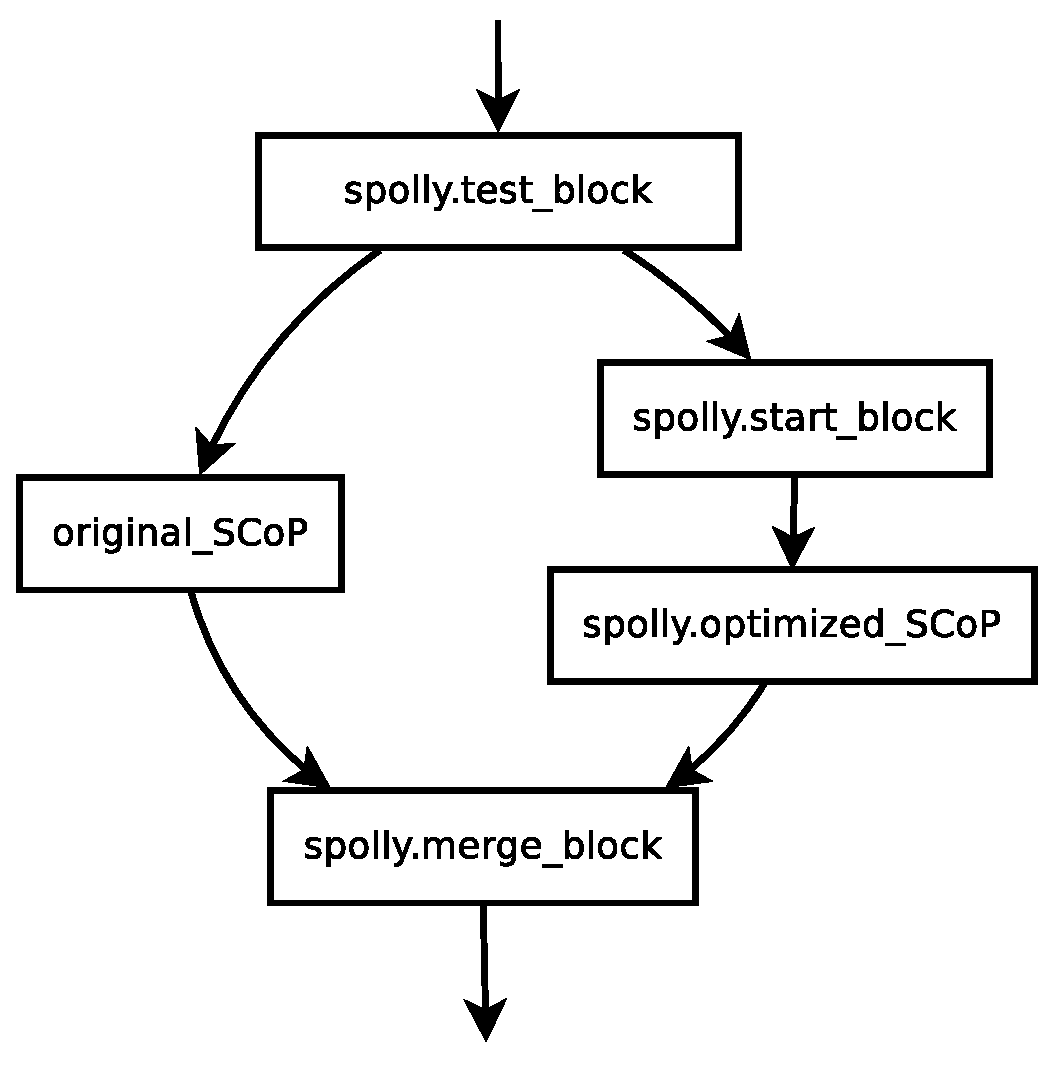
\includegraphics[width=0.45\textwidth]{Figures/SPollySCoPCFG.eps}
  \label{fig:SPollySCoPCFG}}
  \caption{CFG produced by Polly and SPolly, respectively}
  \label{fig:SCoPCFG}  
\end{figure}


\begin{shaded}
\subsubsection{Alias tests} 

Testing for aliasing pointers in general would not be feasible so another way 
was chosen. Only sSCoP invariant pointers are tested once before the sSCoP is
entered. If the test succeeds, thus no aliases are found, the optimized version
is executed. At compile time all accesses for each base pointer are gathered and
marked as possible minimal, possible maximal and not interesting access. At 
runtime all possible minimal and maximal, respectively, accesses are compared 
and the minimal and maximal access for each base pointer is computed. The test 
itself compares again the minimal access for a base pointer with the maximal 
accesses for the others and vice versa. At the end of this comparison chain the 
result replaces the constant guard in the split block before the original SCoP 
and the speculative optimized one. If all base pointers are invariant in the
SCoP the test is complete, thus aliasing can be ruled out for the sSCoP at
runtime. Figure \ref{fig:AliastestConcept} illustrates the concept of the alias
tests while listing \ref{lst:AliastestAccessesSrc} and figure
\ref{fig:AliastestAccesses} provide an example with the derived accesses. 

\end{shaded}


\begin{figure}[htbp]
  \centering
  \subfloat[Alias test from a birds eye view]{
  \includegraphics[width=0.9\textwidth]{Primitives/aliastest.eps}
  \label{fig:AliastestConcept}  
  }

  \lstset{frame=none}
  \subfloat[Aliasing accesses]{
  \lstinputlisting{Primitives/Code/aliastestbsp.c}
  \label{lst:AliastestAccessesSrc}  
  }
  \resetlst
  \hspace*{5mm}
  \subfloat[Statically derived accesses]{
    \begin{tabular}{ c c c c }
      Acc & bp & ma & Ma \\
      \hline
      I1 & C & 0 & N * N \\ 
      I2 & C & 0 & N * N \\ 
      I2 & C & 0 & N * N \\ 
      I3 & A & 0 & N * N \\ 
      I4 & B & 0 & N * N \\ 
    \end{tabular}
    \label{fig:AliastestAccesses}  
  }
  \caption{Alias tests concept}
  \label{fig:Aliastest}  
\end{figure}


\begin{shaded}
\subsubsection*{Complete Checks}
Alias tests may rule out aliasing in sSCoPs completely, thus some sSCoPs become
valid SCoPs after this tests are introduced. Such non speculative optimizations
are done by the compile time part of the Sambamba module and may be included in 
Polly too. An example for such an sSCoP is given in figure 
\ref{fig:AliastestBsp}. The presented code is the well known
matrix multiplication example which is a valid SCoP if the arrays do not alias.
For the sake of completeness it is to mention that this code could be
rewritten as array of pointers which would lead to non complete checks. 
Further discussion on different kinds of this example are appended as 
\ref{Appendix1}.


\subsubsection{Invariants tests}
are introduced for score refinement in the profiling versions. The idea is to
monitor changes in sSCoP invariant variables without analysing the call graph 
during runtime. Listing \ref{lst:InvariantTestSRC} gives an example of an sSCoP 
for which invariant tests can be introduced and \ref{lst:InvariantTestOut} shows
the modified source (high level). 

\end{shaded}

\lstset{frame=none}
\begin{figure}[htbp]
  \centering
  \subfloat[source]{
  \lstinputlisting{Primitives/Code/InvariantTestSRC.c}
  \label{lst:InvariantTestSRC}}
  \hspace*{5mm}
  \subfloat[source with invariant tests]{
  \lstinputlisting{Primitives/Code/InvariantTest.c}
  \label{lst:InvariantTestOut}}
  \caption{Invariant test introduced by SPolly}
  \label{lst:InvariantTest}  
\end{figure}
\resetlst



\begin{shaded}
\section{Sambama Compile Time Module}
The compile time part of the Sambamba module locates all sSCoPs
within the given input module and transfers each one afterwards in a separated 
function. These extracted sSCoPs are stored within the created Sambamba 
bitcode or respectively executable file. Extracting every single sSCoP 
decreases the performance but allows to easily change and combine different 
optimized sSCoPs, even if they originated from the same function.   
This minimal functionalities helped to focus on profiling and
execution during runtime, but there is a lot more potential in this part.
Further work could, for example include compile time preparation of sSCoPs.
Imaginable is more than just a precomputed profiling or optimized version of
a sSCoP. As there are a lot of parameters which could have significant impact 
on the performance, several optimized versions of an sSCoP could be created
and stored, in order to choose the best depending on the system and the actual
run, thus depending on runtime information.
While table \ref{tab:PollyOptions} gives an brief
overview of available options for Polly (* means, not accessible from 
command line)
it is not clear which ones will fit best for a particular environment and sSCoP. 
As the method versioning system of Sambamba evolves, the compile time part 
should, in order to reduce the workload at runtime and increase the ability to
adapt. 

\end{shaded}

\red
\begin{shaded}
\section{Sambama Runtime Module}

In addition to the compile time parts, which only rely on static analyses,
the runtime part uses different kinds of runtime information to decide. 
To take advantage of this extra knowledge, most of the decisions, thus most of
the program logic, is implemented in the runtime module. 


Table \ref{}[TODO] gives an overview of the functionalities.

\end{shaded}

\begin{table}[htbp]
  \caption{Functionality of the SPolly Sambamba module}
  \begin{tabular}{| l |}
    \hline
    
    \hline
    \hline

    \hline
  \end{tabular}
\end{table}


\begin{shaded}

\subsection{Profiling}

\end{shaded}

\orange
\begin{shaded}
\section{Profiling For Sambamba}

Sambamba, as heavily developed research project, was not capable of any kind
of profiling when I started my work. By now, there are two profilers available.
The first one, implemented by the authors of Sambamba, 
is used for exact time measuring, while I created the second one to profiles
executions and data.
[TODO if first is used later on, write it here] Both were
developed during the same time to fulfill different needs and could be
[TODO will be ?]  merged anytime soon. 
As most of SPollys parts are unrelated, to both of them, 
the profiling versions, as their name indicates, would become useless without.
This will definitely increase the number of unnecessary created (parallel) 
functions, but it would not render SPolly redundant.
There a sSCoPs which a guarded by sound checks, thus they can be used with the
overhead of only the check. As the use of other sSCoPs could increase the 
performance too, a heuristic could look for promising candidates, even without
any runtime information. This heuristic could be part of future work since even
with a profiler by hand, there are cases where the gathered information
(see [TODO]) are not helpful at all.

\end{shaded}


\begin{table}[htbp]
  \caption{Command line options to interact with SPolly}
  \begin{tabularx}{\textwidth}{ l p{1mm} X  }
    Command line option     && Description  \\
    \hline
    -enable-spolly          && Enables SPolly during SCoP detection,\par
                                (options containing spolly will not work without) \\ 
    -spolly-replace         && Replaces all sSCoPs by optimized versions \par 
                                (may not be sound)  \\
    -spolly-replace-sound   && As spolly-replace, but sound due to runtime checks \par
                                (iff sound checks can be introduced)\\
    -spolly-extract-regions && Extracts all sSCoPs into their own sub function \\
    -polly-forks=N          && Set the block size which is used when 
                             polly-fork-join code generation is enabled\\
    -enable-polly-fork-join && Extracts the body of the outermost,
                             parallelizeable loop, performs loop blocking with
                             block size N and unrolls the new introduced loop 
                             completely \par
                             (one loop with N calls in the body remains)\\
    -polly-inline-forks     && Inline the call instruction in each fork \\
  \end{tabularx}
  \label{tab:CommandLineOptions}
\end{table}

\begin{table}[htbp]
  \caption{Brief overview of Polly's optimization options}
  \begin{tabularx}{\textwidth}{ l p{1mm} X}
    Short or option name          && Description \\
    \hline
    -polly-no-tiling              && Disable tiling in the scheduler  \\
    -polly-tile-size=N\footnote{} && Create tiles of size N \\
    -polly-opt-optimize-only=STR  && Only a certain kind of dependences (all/raw) \\
    -polly-opt-simplify-deps      && Simplify dependences within a SCoP    \\
    -polly-opt-max-constant-term  && The maximal constant term allowed (in the scheduling) \\
    -polly-opt-max-coefficient    && The maximal coefficient allowed (in the scheduling)  \\
    -polly-opt-fusion             && The fusion strategy to choose (min/max) \\
    -polly-opt-maximize-bands     && Maximize the band depth (yes/no) \\
    -polly-vector-width=N\footnotemark[1]  && Try to create vector loops with N iterations \\
    -enable-polly-openmp          && Enable OpenMP parallelized loop creation \\
    -enable-polly-vector          && Enable loop vectorization (SIMD) \\
    -enable-polly-atLeastOnce     && Indicates that every loop is at leas executed once \\
    -enable-polly-aligned         && Always assumed aligned memory accesses \\
    -enable-polly-grouped-unroll  && Perform grouped unrolling, but don't generate SIMD \\
     &&  \\ 
  \end{tabularx}
  \label{tab:PollyOptions}
  \footnotemark[1] Not available from the command line \\
\end{table}


